\chapter{Metody reprezentacji procesów i~decyzji}
\label{cha:podłożeTeoretyczne}
Rozdział dokładniej opisuje pojęcia używane w~tej pracy, które związane są z~procesami biznesowymi. Główny nacisk położony jest na trzy notacje do reprezentacji procesów, decyzji i~cech systemu.

\section{Business Process Model and Notation}
\label{sec:bpmn}
Proces biznesowy to seria działań lub zadań, których wynikiem jest określony rezultat. \emph{BPMN} (\emph{Business Process Model and Notation}) jest notacją stworzoną przez OMG (\emph{Object Managment Group}\footnote{Zobacz: \url{https://www.omg.org/}.}) w~celu graficznej reprezentacji procesów biznesowych za pomocą diagramów stworzonych przy użyciu schematów blokowych. Motorem napędowym do stworzenia tej notacji była potrzeba medium zrozumiałego dla wszystkich użytkowników biznesowych. Tym sposobem notacja \emph{BPMN} jest zrozumiała dla wszystkich interesariuszy, poczynając od analityka biznesowego tworzącego pierwsze szkice procesu, aż po programistów implementujących technologię odpowiedzialną za wykonywanie tych procesów.

\emph{BPMN 2.0}~\cite{BPMN20} jest w~tym momencie najnowszą wersją notacji i~zapewnia ona cztery typy diagramów, aby w~pełni opisać różne aspekty procesów biznesowych:
\begin{itemize}
	\item \textbf{Diagram Kooperacji,}
	\item \textbf{Diagram Współpracy,}
	\item \textbf{Diagram Choreografii,}
	\item \textbf{Diagram Procesów.}
\end{itemize}

Z perspektywy tej pracy, najbardziej interesujący jest ostatni typ diagramów. Jest on najbardziej elementarnym typem i~reprezentuje przepływ sterowania procesu -- w~jakiej kolejności będą wykonywane zadania, podział procesu na osobne przepływy i~sytuacje, które mogą się wydarzyć podczas wykonywania procesu. Poniżej opisane zostały podstawowe elementy, z~których może składać się taki diagram~\cite{BPMNBook}, natomiast rysunek~\ref{fig:bpmnElements} przedstawia graficzną reprezentację opisanych elementów:
\newpage
\begin{itemize}
        \item \textbf{Zdarzenia} -- reprezentują zdarzenia podczas procesu, np. rozpoczęcie procesu. Występują trzy główne typy zdarzeń: początkowe, pośrednie oraz końcowe.
        \item \textbf{Zadania} -- reprezentują prace wykonywaną podczas procesu. Może to być przykładowo zadanie regułowe odpowiedzialne za podjęcie decyzji (połączone z~tabelą decyzyjną w~notacji \emph{DMN}) albo zadanie użytkownika związane z~podaniem pewnych danych.
        \item \textbf{Bramki} -- determinują rozwidlenie i~łączenie przepływu w~procesie. Ich reprezentacja graficzna posiada dodatkowe znaczniki, mówiące o tym, w~jaki sposób przepływ jest kontrolowany:
            \begin{itemize}
                \item \textbf{Bramka równoległa} -- odpowiednik funkcji ,,AND''.
                \item \textbf{Bramka niewykluczająca} -- odpowiednik funkcji ,,OR''.
                \item \textbf{Bramka wykluczająca} -- odpowiednik funkcji ,,XOR''.
            \end{itemize}
        \item \textbf{Przepływy sterowania} -- obrazują relację (połączenia między obiektami).
\end{itemize}
\begin{figure}
    \centering
    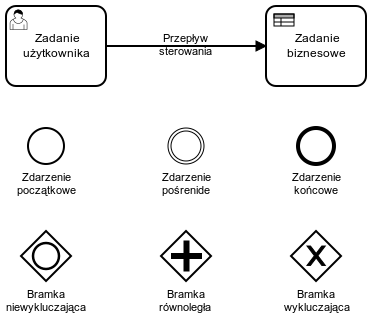
\includegraphics[width=0.6\textwidth, height=0.4\textheight,keepaspectratio]{./assets/bpmnElements.png}
    \caption{Graficzna reprezentacja podstawowych elementów \emph{BPMN}}
    \label{fig:bpmnElements}
\end{figure} 

Rysunek~\ref{fig:bpmnExample} pokazuje przykładowy model procesu w~notacji \emph{BPMN}. Jest on generalnie zrozumiały i~łatwy do analizowania. Ilustruje mały wycinek procesu związanego obsługą złożonego zamówienia przez klienta. Zdarzenie startowe rozpoczyna cały proces. Następnie wykonywane są po kolei dwa zadania. W zależności od danych, które dostarczą te elementy, bramka wykluczająca rozdziela przepływ na dwa. Przepływ górny posiada jedno zadanie, natomiast na przepływie dolnym znowu dochodzi do podziału, tym razem za pomocą bramki równoległej, gdzie wszystkie następujące elementy są wykonywane równolegle. Finalnie przepływy łączą się i~proces jest zakończony przez zdarzenie końcowe. 
\begin{figure}
    \centering
    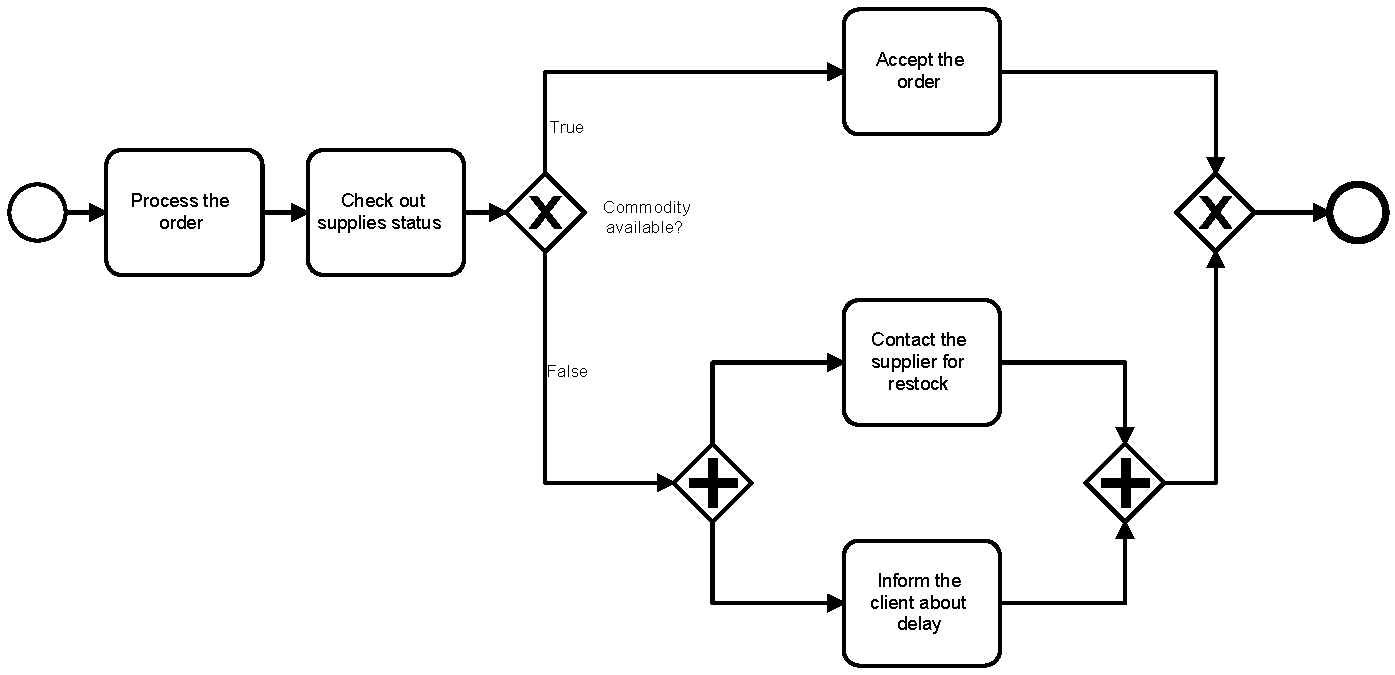
\includegraphics[width=\textwidth]{./assets/processExample.pdf}
    \caption{Przykładowy proces \emph{BPMN}}
    \label{fig:bpmnExample}
\end{figure}

%---------------------------------------------------------------------------
\section{Decision Model and Notation}
\label{sec:dmn}
\emph{DMN} (\emph{Decision Model and Notation}) jest notacją stworzoną przez OMG w~celu prostego opisu oraz modelowania reguł występujących w~procesach i~organizacjach. Tak samo jak w~przypadku \emph{BPMN} główną zaletą oraz założeniem tego standardu było umożliwienie prostej komunikacji użytkowników z~dziedzin biznesu oraz IT. Dzięki niemu bezproblemowa staje się współpraca pomiędzy ludźmi biznesu monitorującymi i~zarządzającymi decyzjami, analitykami biznesowymi, którzy szkicują wstępne wymagania decyzyjne wraz z~logiką decyzyjną oraz technicznymi programistami odpowiedzialnymi za implementację systemów, które te decyzje podejmują. Standard ten może być używany jako samodzielny, jednak najczęściej towarzyszy on notacji \emph{BPMN}. \emph{BPMN} definiuje zadanie regułowe, które może być połączone z~odpowiednim obiektem w~notacji \emph{DMN}. Dzięki temu reguły biznesowe mogą być wcielone do wykonywalnych procesów i~wraz z~działaniem przetwarzać dane oraz odpowiednio ewaluować decyzje.

\emph{DMN 1.2}~\cite{DMN12} jest w~tym momencie najnowszą wersją notacji i~definiuje on cztery elementy:
\begin{itemize}
    \item \textbf{Diagram wymagań decyzyjnych} -- diagram pokazujący zależności między elementami w~notacji \emph{DMN}. Określa on wymagania dla logiki decyzyjnej.
    \item \textbf{Kontekst biznesowy} -- kontekst decyzji, np. jak duży wpływ mają decyzje na wskaźniki wydajności lub jaka jest ich rola.
    \item \textbf{FEEL (\emph{Friendly Enough Expression Language})} -- język służący do określania reguł biznesowych w~tabelach decyzyjnych lub innych logicznych formatach.
    \item \textbf{Logika decyzyjna} -- logika będąca wewnątrz obiektów występujących w~\emph{diagramie wymagań decyzyjnych}. W kontekście tej pracy głównie będzie się to odnosić do tabel decyzyjnych.
\end{itemize}

Diagram wymagań decyzyjnych jest zbudowany bardzo podobnie do diagramu w~notacji \emph{BPMN}. Podstawowe obiekty, z~których się składa opisane zostały poniżej~\cite{DMNArticle}, natomiast rysunek~\ref{fig:dmnElements} przedstawia ich graficzną reprezentację:
\begin{itemize}
    \item \textbf{Elementy}
        \begin{itemize}
            \item \textbf{Decyzje} -- elementy determinujące wynik na podstawie pewnej ilości danych poprzez aplikowanie logiki decyzyjnej. 
            \item \textbf{Dane wejściowe} -- zewnętrzne dane, niepochodzące z~\emph{kontekstu biznesowego}. 
            \item \textbf{Źródła wiedzy} -- źródła określające reguły podejmowania decyzji. Przykładem może być tutaj polityka firmy lub regulacja.
            \item \textbf{Wiedza biznesowa} -- pewne funkcje, które enkapsulują logikę decyzyjną (reguły biznesowe, tablice decyzyjne). Powinny one być łatwe do wielokrotnego użycia.
        \end{itemize}
    \item \textbf{Wymagania}
        \begin{itemize}
            \item \textbf{Wymagania dotyczące informacji} -- połączenia wskazujące dane wejściowe oraz decyzje.
            \item \textbf{Wymagania dotyczące wiedzy} -- połączenia wskazujące jaki model wiedzy biznesowej będzie wykorzystywany w~procesie podejmowania decyzji.
            \item \textbf{Umocowanie wymagania} -- połączenia wskazujące, które z~elementów są źródłami wiedzy.
        \end{itemize}
\end{itemize}
\begin{figure}
    \centering
    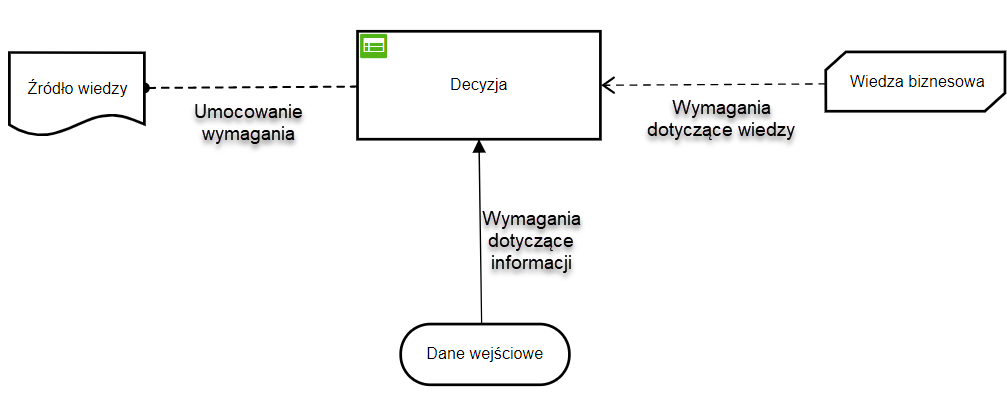
\includegraphics[width=\textwidth,height=0.4\textheight,keepaspectratio]{./assets/dmnElements2.png}
    \caption{Graficzna reprezentacja elementów \emph{diagramu wymagań decyzyjnych}}
    \label{fig:dmnElements}
\end{figure}

Rysunek~\ref{fig:dmnTable} opisuje przykładową tablicę decyzyjną. Warto zauważyć użycie \emph{FEEL} -- przykładowo~w~kolumnie OrderSize można~w~prosty sposób uzależnić zwracaną wartość od tego, czy dostarczone dane będą mniejsze lub większe od liczby dziesięć.
\begin{figure}
    \centering
    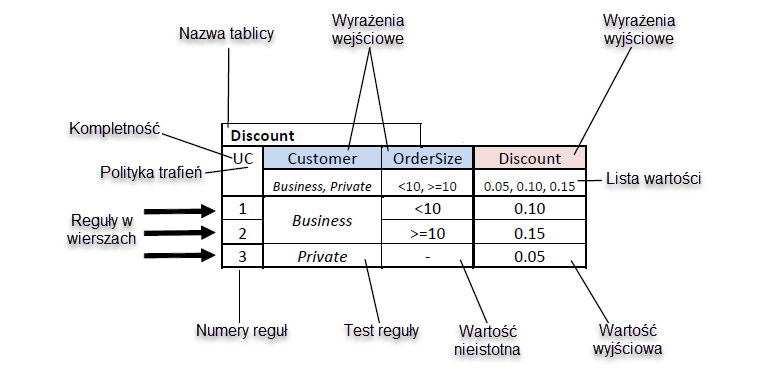
\includegraphics[width=\textwidth]{./assets/dmnTable.png}
    \caption{Tablica decyzyjna w~notacji \emph{DMN}~\cite{DMNTable}}
    \label{fig:dmnTable}
\end{figure}

Rysunek~\ref{fig:dmnExample} prezentuje jak w~praktyce wygląda integracja opisanych standardów. Zadanie regułowe w~procesie zbudowanym za pomocą notacji \emph{BPMN} jest połączone z~decyzją w~notacji \emph{DMN}. Ta z~kolei posiada pewną logikę -- reguły biznesowe wyrażone za pomocą tabeli decyzyjnej i~na tej podstawie, podczas działania procesu, ewaluuje decyzję. 
\begin{figure}
    \centering
    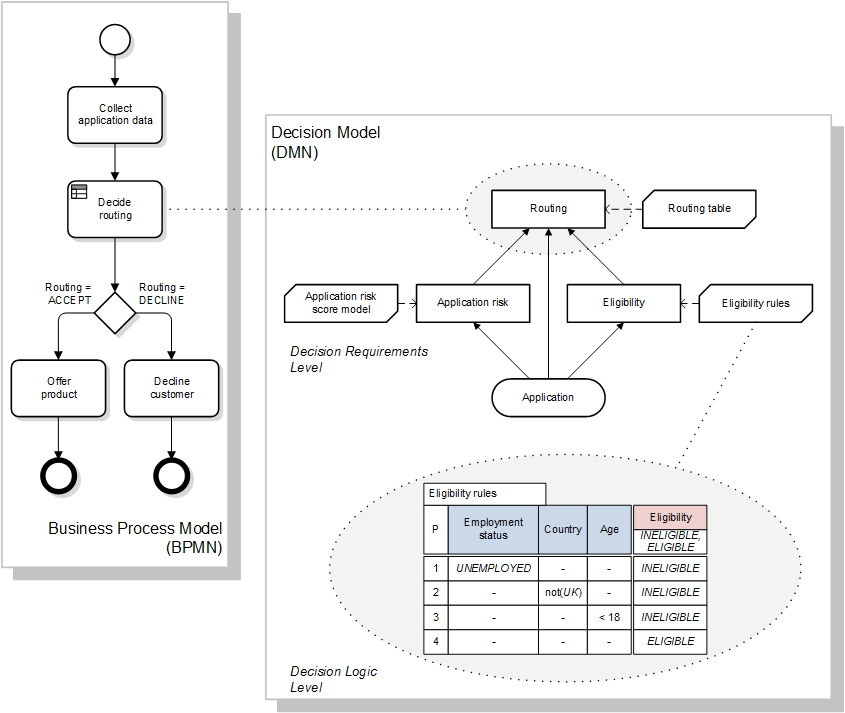
\includegraphics[width=\textwidth,height=0.4\textheight,keepaspectratio]{./assets/dmnExample.png}
    \caption{Integracja modelu \emph{BPMN} oraz \emph{DMN}~\cite{DMN12}}
    \label{fig:dmnExample}
\end{figure}

%---------------------------------------------------------------------------
\section{Attribute Relationship Diagrams}
\label{sec:ard}
\emph{ARD} (\emph{Attribute Relationship Diagrams}) to metoda, której celem jest przedstawienie relacji pomiędzy pewnymi atrybutami danego systemu. Wspomniane atrybuty są elementami branymi pod uwagę w~przypadku rozważania logiki biznesowej. Z początku metoda \emph{ARD} była zaproponowana jako mechanizm prototypowania baz wiedzy, głównie wykorzystywanych w~silnikach regułowych~\cite{ARDFirst}. Działanie miało być podobne do generowania struktur relacyjnych baz danych na podstawie diagramów ER\footnote{Więcej na temat \emph{ERD}: \url{http://citeseerx.ist.psu.edu/viewdoc/download?doi=10.1.1.526.369&rep=rep1&type=pdf}.} (\emph{Entity-Relationship Diagrams}). W kontekście tej pracy \emph{ARD} jest odpowiedzią na problem związany z~prototypowaniem modeli procesów biznesowych. Oferuje ona prosty sposób na szybkie tworzenie szkiców, z~których następnie system potrafi stworzyć bardziej skomplikowane struktury w~notacjach \emph{BPMN} oraz \emph{DMN}. Proces tworzenia modelu \emph{ARD} jest prosty i~iteracyjny, co przyczynia się do zwiększania szczegółowości modelu z~każdym kolejnym krokiem. Całość opiera się na przechodzeniu od ogólnej koncepcji do bardzo szczegółowego modelu\footnote{Rozumowanie dedukcyjne -- ,,od ogółu do szczegółu''.}, jednocześnie zachowując funkcjonalne zależności pomiędzy poszczególnymi elementami.

Diagram \emph{ARD} jest zbiorem pewnych własności i~zależności między nimi. Elementy, z~których jest zbudowany to:
\begin{itemize}
    \item \textbf{Własność} -- własność, która reprezentuje pewne atrybuty. Własności można podzielić na proste i~złożone. Każda zależność może być zależna (zależeć od innej własności) lub niezależna.
        \begin{itemize}
            \item \textbf{Prosta} -- własność prosta reprezentuje jeden atrybut. Takiej własności nie da się podzielić na pewien zbiór własności, jest atomiczna. Przykładem takiej własności może być wiek lub wzrost, są to własności reprezentujące dokładnie jeden atrybut.
            \item \textbf{Złożona} -- własność złożona, reprezentuje zbiór atrybutów. Da się ją podzielić na zbiór prostych własności. Przykładem takiej własności mogą być ,,pomiary'' -- jest to własność, która wewnątrz może kryć wiele atrybutów, takich jak np. wzrost, waga.  
        \end{itemize} 
    \item \textbf{Zależność} -- zależność łączy ze sobą własności i~pokazuje relację między nimi. 
\end{itemize}

Rysunek~\ref{fig:ardExample} prezentuję prosty diagram \emph{ARD}. Występują na nim dwie własności. ,,Pomiary'' jest własnością niezależną. Możliwym byłoby zastąpienie jej wartościami typu waga oraz wzrost. ,,Wartość BMI'' jest własnością zależną, więc nie jest możliwe ewaluowanie jej bez poprzedniego określenia własności źródłowych.
\begin{figure}
    \centering
    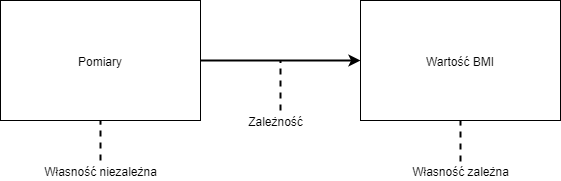
\includegraphics[width=0.6\textwidth]{./assets/ardExample.png}
    \caption{Przykład prostego diagramu \emph{ARD}}
    \label{fig:ardExample}
\end{figure}

Jasno widać, że nietrudnym zadaniem byłoby rozbudowanie takiego diagramu o kolejne własności\linebreak i~to jest główną zaletą tej metody -- prostota i~iteracyjna natura. Aby lepiej zobrazować proces tworzenia diagramu \emph{ARD} warto pochylić się nad konkretnym przykładem, wykorzystując jednocześnie diagram z~rysunku~\ref{fig:ardExample}. Niech przykładową sytuacją będzie potrzeba naszkicowania, przez analityka biznesowego, prototypu modelu związanego z~poradami zdrowotnymi. Model ma opierać się na BMI (\emph{Body Mass Index\footnote{Więcej na temat \emph{BMI}: \url{https://www.researchgate.net/publication/276444598_Body_Mass_Index}.}}). Wykorzystując wcześniej wspomniany iteracyjny proces, finalną własnością byłaby porada zdrowotna i~z~każdą kolejną iteracją analityk wprowadzałby coraz to nowsze i~bardziej szczegółowe własności, budując w~taki sposób diagram zależności. Porada potrzebowałaby imienia pacjenta oraz jego poziomu \emph{BMI}. Do obliczenia poziomu \emph{BMI} potrzebna by była płeć pacjenta oraz wartość \emph{BMI}. Natomiast sama wartość byłaby obliczana na podstawie wagi oraz wzrostu. Finalny wykres i~opisane rozumowanie obrazuje rysunek~\ref{fig:ardComplexExample}.
\begin{figure}
    \centering
    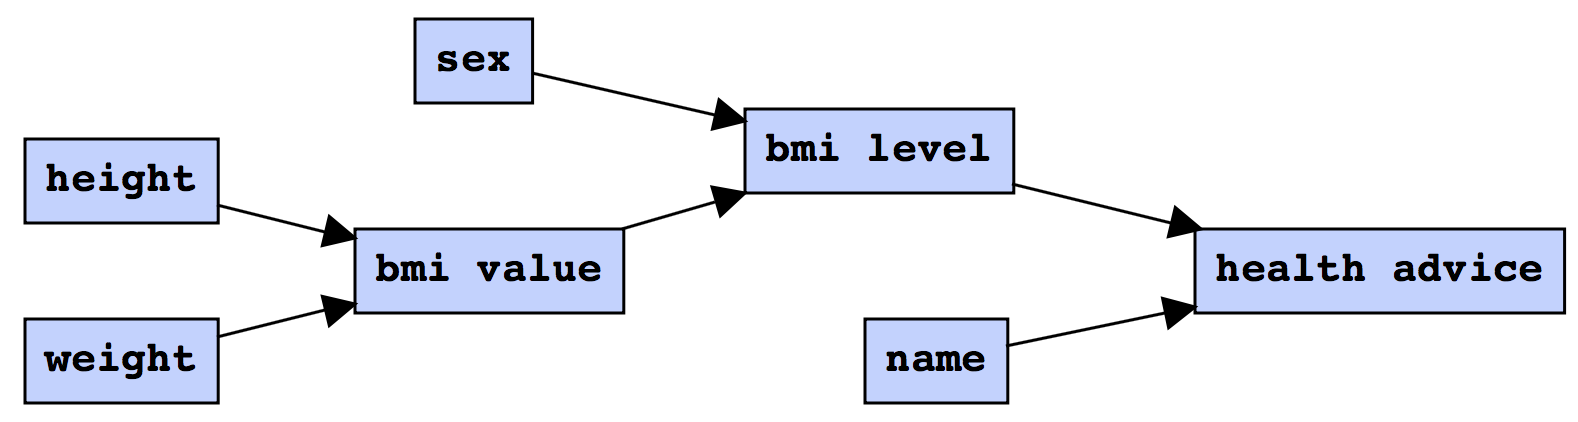
\includegraphics[width=\textwidth]{./assets/ardComplexExample.png}
    \caption{Diagram \emph{ARD} dla modelu związanego z~poradą zdrowotną~\cite{ARDtoBPM}}
    \label{fig:ardComplexExample}
\end{figure}

Wykorzystując dalej przykład z~rysunku~\ref{fig:ardComplexExample} oraz mając na uwadze wcześniej opisane standardy \emph{BPMN} oraz \emph{DMN}, można pokusić się o przeniesienie tego prototypu do wspomnianych notacji. Rysunek~\ref{fig:ardBPMDMNFinal} prezentuje koncepcję takiej operacji. Wystarczyłoby odpowiednio pogrupować własności i~ich zależności, przedstawić każdą własność prostą jako zadnie użytkownika, w~którym użytkownik musi podać dane, a~każdą własność złożoną jako zadanie biznesowe, czyli zadanie połączone z~decyzją (gdzie wykorzystywana jest tablica decyzyjna). Na wspomnianym rysunku przykładem zadania użytkownika jest ,,Enter Measures'', które dostarcza ,,height'' oraz ,,width'' do tablic decyzyjnych, a~przykładem zadania biznesowego jest ,,Determine bmi level''.
\begin{figure}
    \centering
    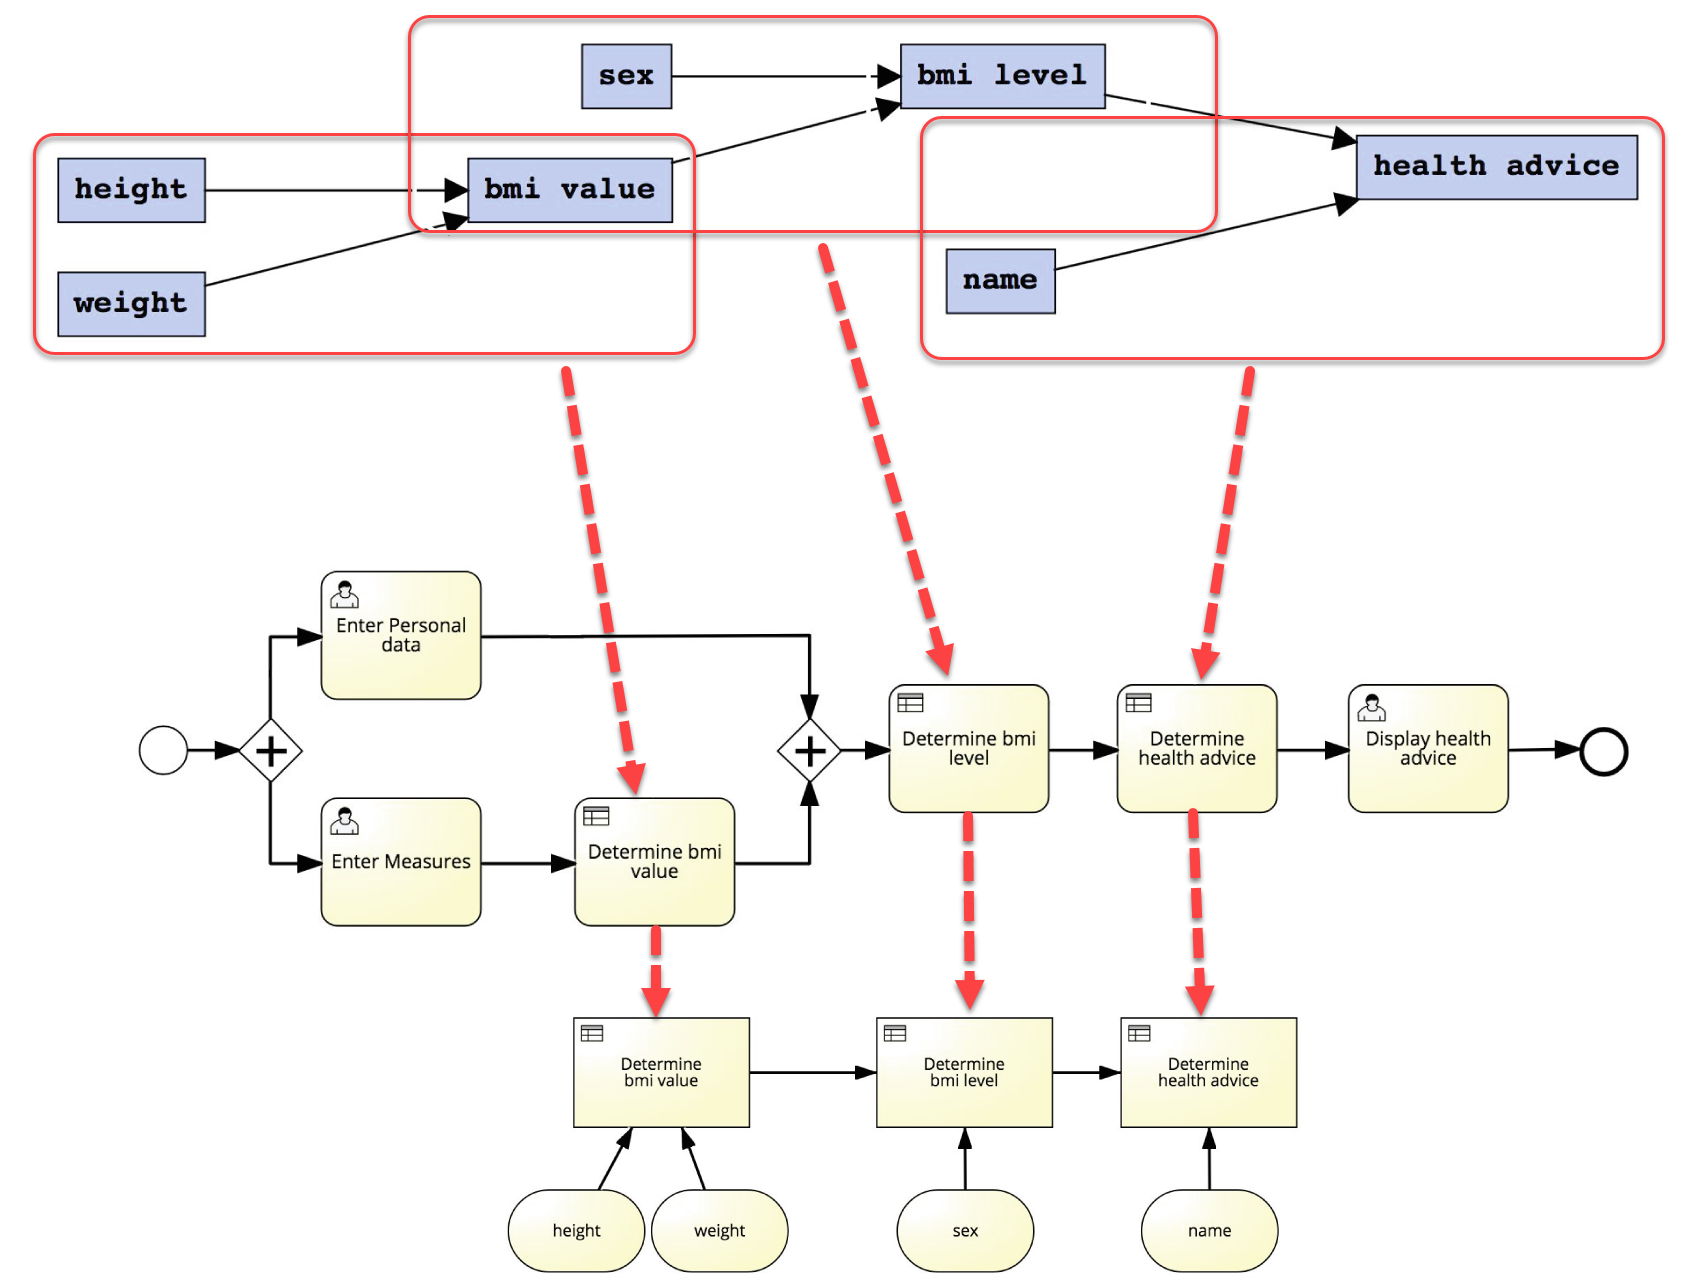
\includegraphics[width=\textwidth,height=0.4\textheight,keepaspectratio]{./assets/ardBPMDMNFinal.png}
    \caption{Koncept transformacji diagramu \emph{ARD} do modelu w~notacji \emph{BPMN} oraz \emph{DMN}~\cite{ARDtoBPM}}
    \label{fig:ardBPMDMNFinal}
\end{figure} 

%---------------------------------------------------------------------------
\subsection{Hekate Markup Langauge}
\label{sec:hml}
\emph{HML} (\emph{Hekate Markup Language}) to język stworzony do reprezentacji bazy reguł \emph{HeKatE\footnote{Więcej na temat \emph{HeKatE}: \url{https://ai.ia.agh.edu.pl/hekate:start}.}}, zapisanych formacie HMR (\emph{Hekate Meta Representation\footnote{Więcej na temat \emph{HMR}: \url{https://ai.ia.agh.edu.pl/hekate:hmr}.}}). Język \emph{HML} posiada trzy podzbiory:
\begin{itemize}
    \item \textbf{attml} -- Attribute Markup Language opisujący atrybuty reguł,
    \item \textbf{ardml} -- Attribute Relationship Markup Language służący do ekspresji prototypów w~ARDplus (rozszerzeniu \emph{ARD}),
    \item \textbf{xttml} -- XTT2 Rule Markup Language służący do reprezentacji ustrukturyzowanych reguł XTT2\footnote{Więcej na temat \emph{XTT2}: \url{https://ai.ia.agh.edu.pl/hekate:xtt2}.}.
\end{itemize}
W zależności od potrzeb, możliwe jest różnorakie wykorzystanie opisanych podjęzyków:
\begin{itemize}
    \item \textbf{attml} -- tylko definicje atrybutów (minimalistyczny przypadek),
    \item \textbf{attml + ardml} -- atrybuty oraz zależności \emph{ARD}, 
    \item \textbf{attml + ardml + xttml} -- atrybuty, zależności oraz reguły \emph{XTT2},
    \item \textbf{attml + xttml} -- atrybuty i~reguły (bez prototypu \emph{ARD}).
\end{itemize}\newpage
Listing~\ref{lst:hmlFileExample} prezentuje strukturę pliku \emph{HML} wykorzystującego wszystkie wspomniane podjęzyki. 
\lstinputlisting[language=XML, caption={Przykład struktury pełnego pliku \emph{HML}}, label={lst:hmlFileExample}]{./listings/hmlFileExample.xml}

Składnia wymaga, aby wszystkie ważne elementy posiadały atrybut ,,id'', będący unikatowym identyfikatorem. Dodatkowo każdy element powinien zawierać odpowiedni przedrostek:
\begin{itemize}
    \item \texttt{types} -- identyfikator powinien zaczynać się od ,,tpe'',
    \item \texttt{attributes} -- identyfikator powinien zaczynać się od ,,att'',
    \item \texttt{properties} -- identyfikator powinien zaczynać się od ,,prp'',
    \item \texttt{type groups} -- identyfikator powinien zaczynać się od ,,tgr'',
    \item \texttt{attribute groups} -- identyfikator powinien zaczynać się od ,,agr'',
    \item \texttt{dependencies} -- identyfikator powinien zaczynać się od ,,dep'',
    \item \texttt{ARD history} -- identyfikator powinien zaczynać się od ,,hst''.
\end{itemize}

W kontekście niniejszej pracy pliki \emph{HML}, które będą brane pod uwagę, powinny zawierać w~sobie podzbiór językowy \emph{ardml}, jednak z~opcjonalnym fragmentem \emph{TPH}, gdyż nie jest on wykorzystywany przy tworzeniu modelu procesu finalnego. Przykład wymaganego pliku prezentuje listing~\ref{lst:ardmlExample}.
\lstinputlisting[language=XML, caption={Przykład struktury pliku \emph{HML} z~podzbiorem \emph{ardml}}, label={lst:ardmlExample}]{./listings/ardmlExample.xml}
\vspace{1cm}

Jest to koniec rozdziału opisującego metody reprezentacji procesów i~decyzji. W tym rozdziale opisane zostały najważniejsze terminy, które będą często pojawiać się w~dalszej części niniejszej pracy. W~kolejnym rozdziale zostanie przedstawiony projekt aplikacji, która wykorzystuje opisane tutaj notacje \emph{BPMN}, \emph{DMN} oraz \emph{ARD}.

